\chapter{Исследовательская часть}

В данном разделе будет приведен пример работы программы, а также проведен сравнительный анализ алгоритмов при различных ситуациях на основе полученных данных.

\section{Технические характеристики}

Технические характеристики устройства, на котором выполнялся эксперимент представлены далее:

\begin{enumerate}[label=\arabic*)]
	\item операционная система --- Ubuntu 22.04.3~\cite{ubuntu} Linux x86\_64;
	\item память --- 16 Гб;
	\item процессор --- четырехъядерный процессор Intel® Core™ i5-1135G7 @ 2.40 ГГц.
\end{enumerate}

При эксперименте ноутбук не был включен в сеть электропитания.

\section{Демонстрация работы программы}

На рисунке~\ref{fig:example} представлен интерфейс программы.

\begin{figure}[h!]
	\centering
	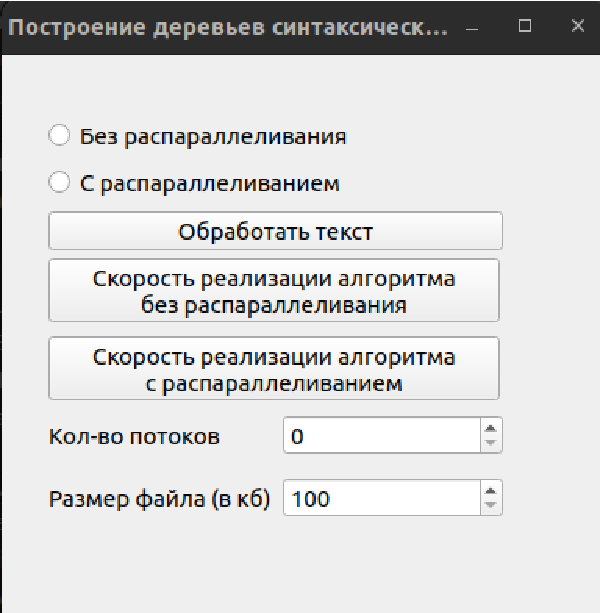
\includegraphics[width=0.4\linewidth]{img/example}
	\caption{Пример работы программы}
	\label{fig:example}
\end{figure}

\section{Время выполнения реализаций алгоритмов}

Как было сказано выше, используется функция замера процессорного времени \textit{std::chrono::system\_clock::now(...)} из библиотеки $chrono$ на C++. Функция возвращает процессорное время типа float в секундах.

Функция используется дважды: перед началом выполнения алгоритма и после завершения, затем из конечного времени вычитается начальное, чтобы получить результат.

Замеры проводились для файлов с текстом размером от 100 до 1000 кб, без дополнительных потоков и с потоками, количество которых от 1 до 32.

Результаты замеров приведены в таблицах \ref{tbl:time_mes_par} и \ref{tbl:time_mes_difdiam} (время в с). А на рисунках \ref{fig:graph_all} и \ref{fig:graph_3} приведены графические результаты замеров.

\begin{figure}[h]
	\centering
	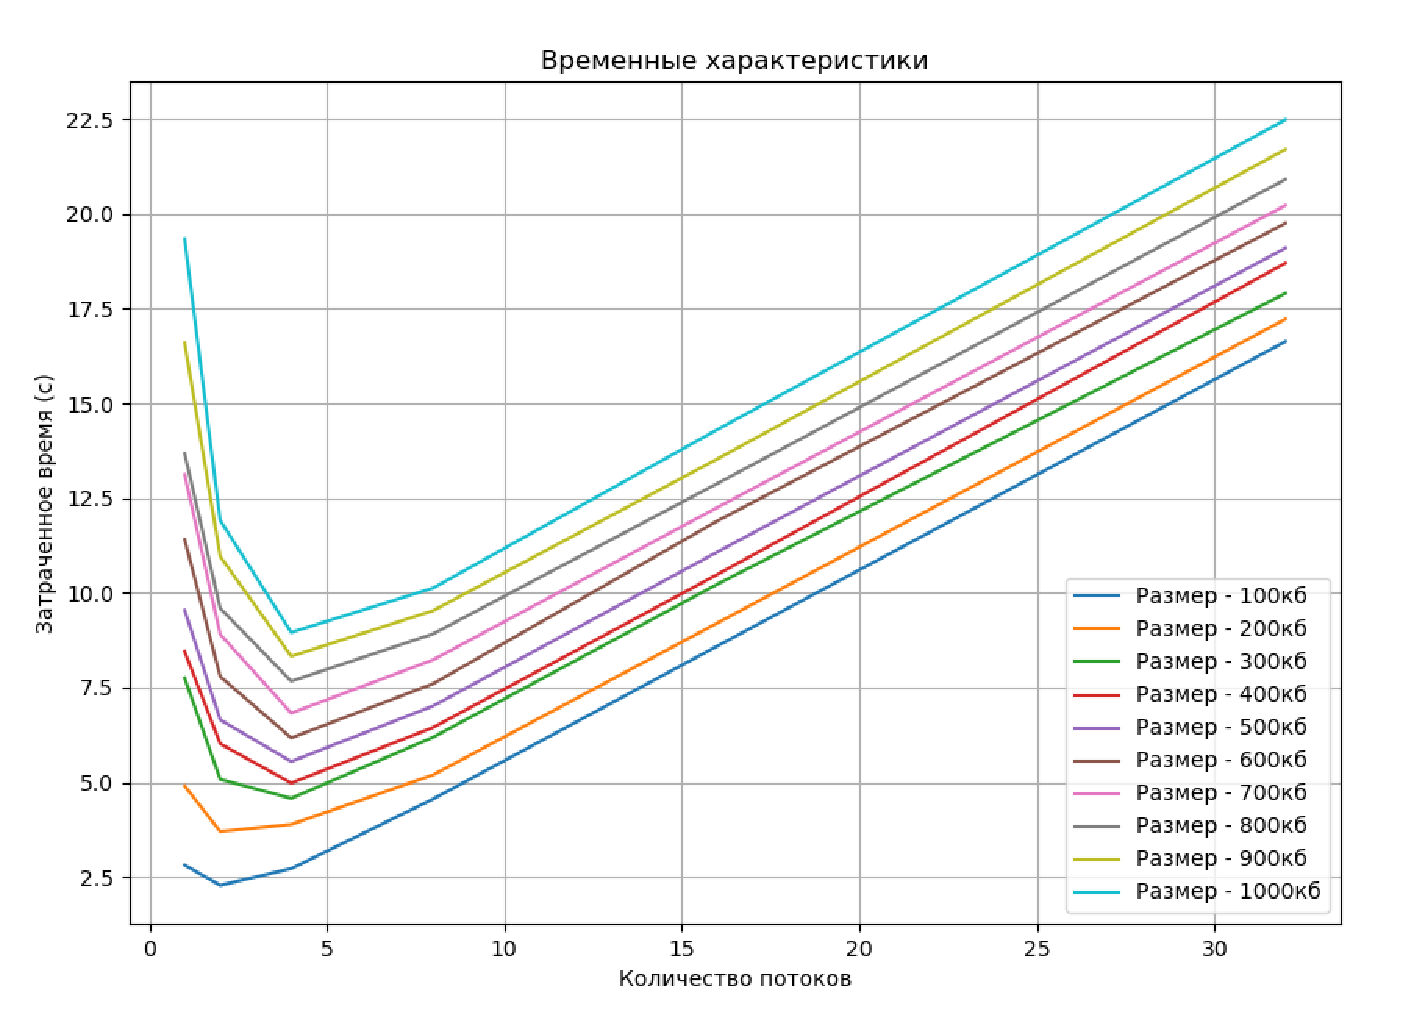
\includegraphics[width=\linewidth]{img/all}
	\caption{Использование разного количества потоков}
	\label{fig:graph_all}
\end{figure}

\begin{figure}[h]
	\centering
	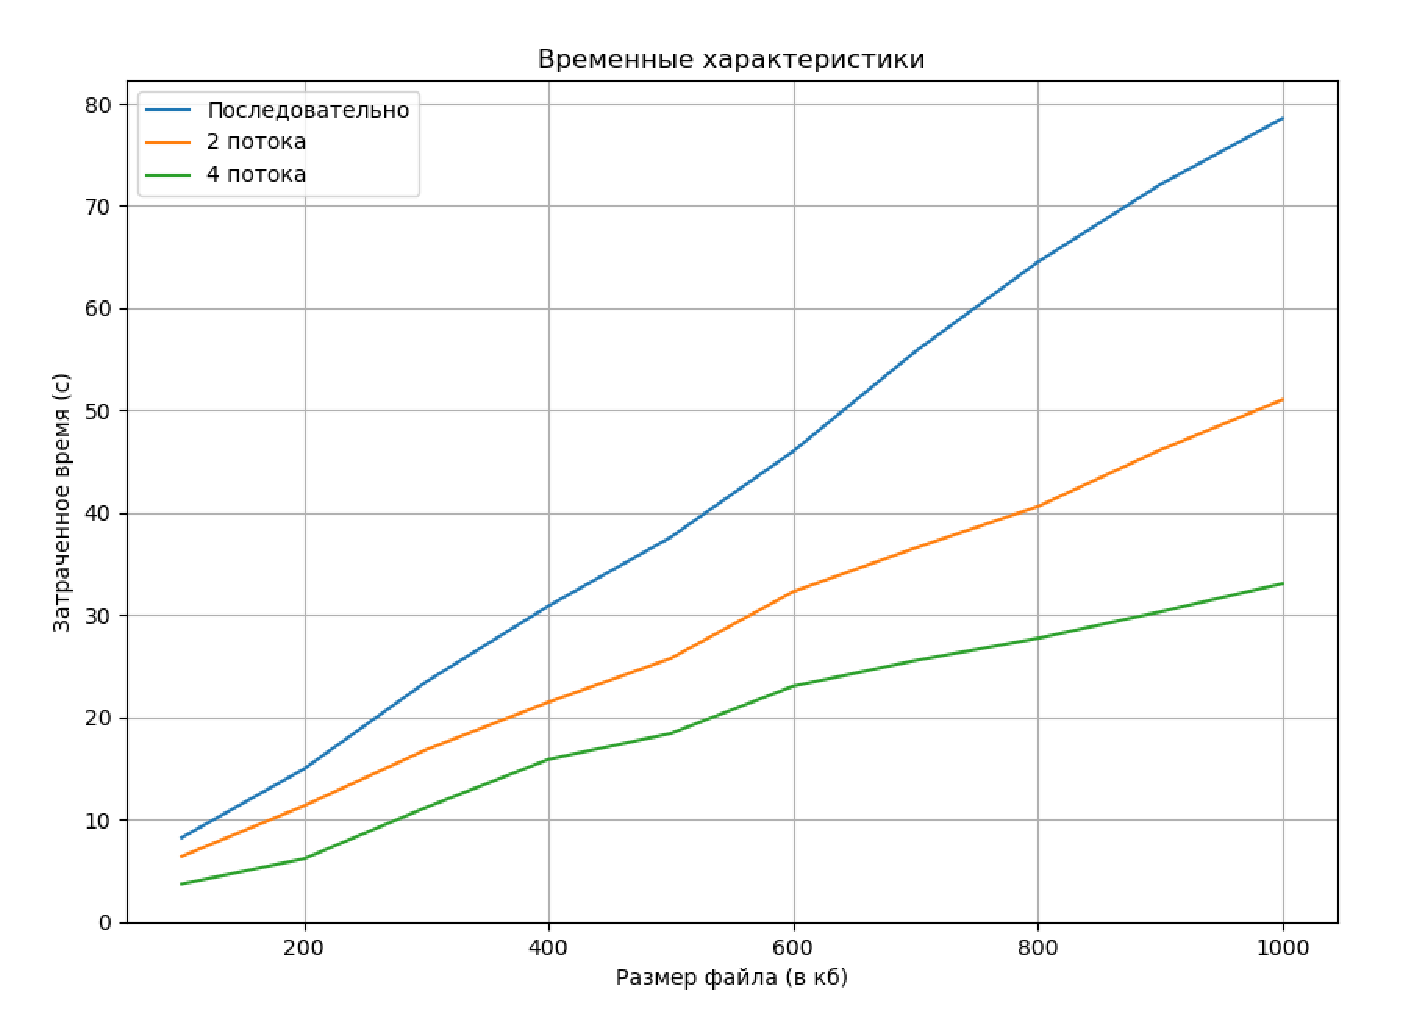
\includegraphics[width=\linewidth]{img/3}
	\caption{Без использования многопоточности и с 2 и 4 потоками}
	\label{fig:graph_3}
\end{figure}

\begin{table}[h]
	\begin{center}
		\begin{threeparttable}
			\captionsetup{justification=raggedright,singlelinecheck=off}
			\caption{Результаты замеров времени (в с) для разного размера файла и разного количества потоков}
			\label{tbl:time_mes_par}
			\begin{tabular}{|c|r|r|r|r|r|r|}
				\hline            
				\multirow{2}{*}{Размер файла (в кб)}& \multicolumn{6}{c|}{Количество потоков} \\
				\cline{2-7}
				& 1 & 2 & 4 & 8 & 16 & 32 \\
				\hline
				100 & 9.15 & 6.40 & 5.54 & 6.10 & 10.91 & 19.33 \\ 
				\hline
				200 & 15.12 & 11.98 & 8.94 & 9.21 & 13.68 & 22.16 \\ 
				\hline
				300 & 25.50 & 16.82 & 11.18 & 13.50 & 17.25 & 24.66 \\ 
				\hline
				400 & 32.59 & 21.47 & 15.87 & 15.07 & 19.83 & 27.90 \\ 
				\hline
				500 & 38.91 & 25.75 & 18.41 & 18.22 & 21.96 & 31.19 \\ 
				\hline
				600 & 48.21 & 32.27 & 23.03 & 21.93 & 24.76 & 34.15 \\ 
				\hline
				700 & 56.33 & 36.55 & 25.54 & 23.50 & 27.54 & 36.38 \\ 
				\hline
				800 & 65.24 & 40.59 & 27.71 & 27.07 & 30.49 & 38.15 \\ 
				\hline
				900 & 73.43 & 46.12 & 30.30 & 27.46 & 32.85 & 42.26 \\ 
				\hline
				1000 & 78.54 & 51.04 & 33.05 & 31.10 & 35.59 & 43.24 \\ 
				\hline
			\end{tabular}
		\end{threeparttable}
	\end{center}
\end{table}

\clearpage

\begin{table}[h]
	\begin{center}
		\begin{threeparttable}
			\captionsetup{justification=raggedright,singlelinecheck=off}
			\caption{Результаты замеров времени без многопоточности}
			\label{tbl:time_mes_difdiam}
			\begin{tabular}{|c|r|}
				\hline
				Размер файла (в кб) & Время (в с) \\
				\hline
				100 & 8.22 \\ 
				\hline
				200 & 14.93 \\ 
				\hline
				300 & 23.47 \\ 
				\hline
				400 & 30.88 \\ 
				\hline
				500 & 37.61 \\ 
				\hline
				600 & 46.00 \\ 
				\hline
				700 & 55.77 \\ 
				\hline
				800 & 64.51 \\ 
				\hline
				900 & 72.08 \\ 
				\hline
				1000 & 78.55 \\ 
				\hline
			\end{tabular}
		\end{threeparttable}
	\end{center}
\end{table}

\section*{Вывод}

В результате эксперимента было получено, что при использовании 4 потоков, время работы многопоточной реализации алгоритма построения деревьев синтаксических зависимостей в тексте меньше, чем время работы реализации без многопоточности в 2.04 раз на размере файла, равном 500 кб. Данное количество потоков обусловлено тем, что на ноутбуке, на котором проводилось тестирование ПО, имеется всего 4 логических ядра. Также важную роль играет то, что работа распределяется примерно равно между всеми потоками, остатки работы отдаются крайнему потоку. При 4 потоках остатка не будет. Именно поэтому лучшие результаты достигаются именно на 4 потоках, даже не смотря на ресурсы, которые дополнительно затрачиваются на содержание потоков. В итоге, можно сказать, что при таких данных следует использовать многопоточную реализацию алгоритма.

Также при проведении эксперимента было выявлено, что при увеличении размера файла, многопоточная реализация выдает все более заметное преимущество по времени перед реализацией без многопоточностью. Так, при размере файла, равном 300 кб многопоточная реализация быстрее реализации без многопоточности в 2.09 раз, а на размере файла, равном 1000 кб --- в 2.37 раз. 

Кроме этого, из эксперимента следует, что реализация с использованием 8 дополнительных потоков работает быстрее, чем с 4 дополнительными потоками при размере файла более 500 кб.